\documentclass[10pt, conference, compsocconf, letterpaper, twocolumn, twoside]{IEEEtran}
\usepackage[utf8]{inputenc}

\usepackage{amsmath}
\usepackage{graphicx}
\usepackage{pgfplots}
\pgfplotsset{compat=1.18}
\title{Enhancing Cybersecurity with Deep Learning: Zero-Day Malware and Intrusion Detection}

% Note: Include both group members as per course requirements
\author{
    \IEEEauthorblockN{Pranav Tej Lalapeta}
    \IEEEauthorblockA{Dept. of Computer Science\\
    University of Central Florida\\
    pr652213@ucf.edu}
    \and
    \IEEEauthorblockN{Sai Karthik Nallamothu}
    \IEEEauthorblockA{Dept. of Computer Science\\
    University of Central Florida\\
    sa808371@ucf.edu}
}

\date{April 2026}

\begin{document}

\maketitle

\begin{abstract}
Sophisticated cyber threats, including zero-day exploits and polymorphic malware, continue to stress signature-centric intrusion detection systems (IDS) that depend on curated indicators of compromise. Such defenses inevitably lag novel attacks, producing a protection gap between first exploitation and manual cataloging of indicators. This paper studies a deep learning--oriented alternative that emphasizes behavioral signals in network traffic rather than static string or hash matching. We compare a dense deep neural network (DNN) for per-flow representation learning, a recurrent model based on long short-term memory (LSTM) cells for temporal context, and a hybrid DNN--RNN stack intended to capture both instantaneous flow statistics and multi-step activity. Evaluation uses the widely adopted NSL-KDD and CICIDS-2017 benchmarks, which mix benign background traffic with diverse attack families. Overall and class-specific results are reported using accuracy, precision, recall, and $F_1$ score so that detection sensitivity can be weighed against analyst-facing false alarms. The empirical trend across both corpora is consistent: hybrid spatial--temporal modeling yields the strongest balance of high recall on difficult classes and stable precision, supporting its role as a complementary analytics layer for security operations centers (SOCs) that must prioritize credible alerts.
\end{abstract}

\begin{IEEEkeywords}
Deep Learning, Intrusion Detection Systems (IDS), Zero-Day Malware, Neural Networks, Network Security, Behavioral Analysis.
\end{IEEEkeywords}

\section{Introduction}
The rapid evolution of the cyber-threat landscape has rendered traditional perimeter-based security measures increasingly obsolete. As organizations migrate toward highly distributed cloud environments and interconnected Internet of Things (IoT) frameworks, the attack surface available to malicious actors has expanded exponentially \cite{buczak2016}. Among these threats, Zero-Day exploits and polymorphic malware represent the most significant challenges to contemporary cybersecurity infrastructure. A Zero-Day vulnerability refers to a software flaw unknown to the vendor, for which no patch or defensive signature has been developed. Because traditional Intrusion Detection Systems (IDS) rely on a library of known "signatures" or hashes to identify threats, they are fundamentally incapable of recognizing these novel attacks during the critical window of initial exposure \cite{denning1987}.

The inadequacy of signature-based detection is further exacerbated by the rise of polymorphic and metamorphic malware. These malicious programs utilize mutation engines to alter their identifiable features—such as file names, encryption keys, and code sequences—each time they replicate. While the underlying malicious intent remains constant, the digital "fingerprint" changes, allowing the malware to bypass traditional antivirus scanners that search for exact matches in a static database \cite{idika2007}. This creates a dangerous "protection gap" where high-value networks remain vulnerable until a human analyst can manually capture, analyze, and catalog the new threat.

Furthermore, modern cyber-attacks are no longer characterized by single, isolated events. Advanced Persistent Threats (APTs) often employ a "low and slow" approach, infiltrating a network and remaining dormant or performing subtle unauthorized actions over several months to exfiltrate sensitive data \cite{alshamrani2019}. Traditional security tools often fail to correlate these temporally distant events, viewing them as isolated, benign occurrences. This lack of contextual awareness leads to significant "alert fatigue" within Security Operations Centers (SOCs). When analysts are inundated with thousands of low-fidelity alerts, the probability of overlooking a genuine breach increases significantly \cite{axelsson2000}.

To address these systemic vulnerabilities, this research proposes a shift toward a behavioral-based defense paradigm powered by Deep Learning (DL). Deep Learning, a subset of machine learning characterized by multi-layered neural networks, offers the unique ability to perform automated feature extraction from raw, high-dimensional data. Unlike traditional machine learning, which requires human experts to manually define what constitutes "malicious" behavior—a process known as feature engineering—Deep Neural Networks (DNNs) can autonomously identify non-linear patterns and correlations within network traffic that are invisible to human observers \cite{lecun2015}.

Specifically, this study explores the integration of Recurrent Neural Networks (RNNs) to provide the temporal "memory" necessary to detect multi-stage attacks. By training these models on standardized benchmarks such as the CICIDS-2017 and NSL-KDD datasets, we aim to establish a system that does not ask, "Does this file match a known threat?" but rather, "Does this behavior deviate from the statistical baseline of a healthy network?" \cite{sharafaldin2018}. The goal of this project is to evaluate the performance of these architectures in terms of accuracy, precision, and recall, ultimately providing a blueprint for an automated, proactive cybersecurity posture.

\section{Literature Review}
The application of Artificial Intelligence (AI) to network security has transitioned from theoretical exploration to operational necessity. Early literature focused on signature-based systems, but as the complexity of malware increased, research pivoted toward anomaly detection. This section analyzes the progression of research through 15 key studies from IEEE and ACM repositories.

\subsection{Transition from Shallow to Deep Learning}
Early efforts in Intrusion Detection Systems (IDS) utilized shallow machine learning models. Studies by Buczak and Guven \cite{buczak2016} provided a foundational survey of data mining methods, noting that while Support Vector Machines (SVM) and Random Forests were effective for known patterns, they struggled with high-dimensional "noisy" data. Sommer and Paxson \cite{sommer2010} famously critiqued the "closed world" assumption of machine learning in security, arguing that anomaly detection often fails in production due to the extreme variability of benign traffic.

The breakthrough for Deep Learning (DL) in this field came with the ability to perform automated feature extraction. Kim et al. \cite{kim2016} utilized Long Short-Term Memory (LSTM) networks to capture the temporal dependencies of network flows, outperforming traditional RNNs in detecting long-duration attacks. Similarly, Yin et al. \cite{yin2017} demonstrated that deep architectures inherently solve the feature engineering bottleneck that plagued previous generations of IDS research.

\subsection{Dataset Evolution and Benchmarking}
The validity of any AI-driven security research is intrinsically linked to the underlying data. The KDD Cup '99 dataset was the primary benchmark for over a decade, but Tavallaee et al. \cite{tavallaee2009} conducted a seminal study highlighting its critical flaws, including redundant records that caused models to overfit on frequent but harmless patterns. This led to the development of the NSL-KDD dataset, which improved the balance between benign and malicious traffic.

However, even NSL-KDD lacked modern attack representations. To modernize benchmarking, Sharafaldin et al. \cite{sharafaldin2018} introduced the CICIDS-2017 dataset, which captured diverse attack profiles such as DoS, Brute Force, and Infiltration using the B-Profile system. Recent comparative analyses by Ferrag et al. \cite{ferrag2020} and Hindy et al. \cite{hindy2020} suggest that while newer datasets like CSE-CIC-IDS2018 provide more volume, the 2017 version remains the gold standard for evaluating model precision in academic settings.

\subsection{Architectural Innovations and Hybrid Models}
Recent ACM publications have explored hybridizing different neural architectures to minimize False Positive Rates (FPR). Zhang et al. \cite{zhang2019} proposed a hierarchical model that combines Convolutional Neural Networks (CNNs) for spatial packet analysis and Gated Recurrent Units (GRUs) for temporal flow analysis. This dual-stream approach proved significantly more resilient against "low and slow" Advanced Persistent Threats (APTs).

Moreover, the integration of Autoencoders (AE) for unsupervised learning has gained traction. Javaid et al. \cite{javaid2016} utilized Deep Belief Networks (DBN) for self-taught learning, proving that models could identify anomalies even when the training data was partially unlabeled. This was further refined by Otoum et al. \cite{otoum2019}, who compared Restricted Boltzmann Machines (RBM) against traditional DL models, finding that hybrid-RL (Reinforcement Learning) models offered better adaptability to dynamic network changes.

\subsection{The Adversarial Frontier}
A growing body of research addresses the vulnerability of the models themselves. Biggio and Roli \cite{biggio2018} provided a comprehensive review of adversarial machine learning, noting that attackers can "poison" IDS training data or use "evasion attacks" to find mathematical blind spots in the classifier. Current research by Yuan et al. \cite{yuan2019} in IEEE Access explores the use of Generative Adversarial Networks (GANs) to generate "adversarial malware" that can bypass even the most advanced deep learning detectors, highlighting the need for robust, defensive distillation techniques in future IDS designs.

\section{Proposed Methodology}
The proposed framework is engineered to move beyond the limitations of static analysis by treating network traffic as a high-dimensional, time-varying signal. The methodology is structured into a logical pipeline consisting of four primary stages: Data Acquisition, Multi-Stage Preprocessing, Hybrid Neural Architecture Design, and Optimization.

\subsection{Standardized Dataset Integration}
For a robust evaluation, we utilize the \textbf{CICIDS-2017} and \textbf{NSL-KDD} datasets. These provide the necessary diversity to train a generalized model.
\begin{itemize}
    \item \textbf{Benign Baseline:} Establishing a statistical "norm" for the network using standard protocols (HTTP, HTTPS, SSH).
    \item \textbf{Malicious Vectors:} Training the model on diverse attack profiles, including DDoS, Brute Force, Heartbleed, and Botnets, to ensure the system recognizes the behavioral signatures of Zero-Day exploits.
\end{itemize}

\subsection{The Preprocessing Pipeline}
Raw network data is inherently heterogeneous and cannot be directly ingested by neural layers. We implement a rigorous three-step preprocessing sequence:
\begin{enumerate}
    \item \textbf{Feature Selection and Sanitization:} We remove non-generalizable metadata, such as specific IP addresses and timestamps. This prevents "overfitting," where the model simply memorizes the source of an attack rather than learning the underlying malicious behavior.
    \item \textbf{One-Hot Encoding for Categorical Data:} Non-numerical features (e.g., Protocol Type: TCP, UDP, ICMP) are transformed into binary vectors. This prevents the network from assuming a false numerical hierarchy between protocols.
    \item \textbf{Min-Max Scaling and Normalization:} Because features like "Packet Length" and "Flow Duration" exist on vastly different scales, we normalize all input values to a range of $[0, 1]$ using:
    \begin{equation}
    x_{norm} = \frac{x - x_{min}}{x_{max} - x_{min}}
    \end{equation}
\end{enumerate}

\subsection{Hybrid Neural Architecture Design}
The core of our proposal is a hybrid model that captures both the \textbf{Spatial} and \textbf{Temporal} characteristics of network threats.

\subsubsection{Deep Neural Network (DNN) for Spatial Extraction}
The DNN serves as the primary classifier for individual flow characteristics. 
\begin{itemize}
    \item \textbf{Layered Funneling:} We implement a three-layer dense architecture (128-64-32 neurons). This reductionist design forces the network to learn compressed, abstract representations of the data.
    \item \textbf{ReLU Activation:} The Rectified Linear Unit, $f(x) = \max(0, x)$, is applied to each hidden layer to ensure rapid convergence and prevent gradient stagnation.
    \item \textbf{Dropout Regularization:} To harden the model against never-before-seen Zero-Days, a 20\% dropout rate is applied, forcing the network to develop redundant detection pathways.
\end{itemize}

\subsubsection{Recurrent Neural Network (RNN) with LSTM Cells}
To detect multi-stage Advanced Persistent Threats (APTs), we integrate Long Short-Term Memory (LSTM) units. Unlike standard DNNs, LSTMs maintain a "cell state" ($C_t$) that tracks the history of a connection. This allows the system to correlate a suspicious login attempt with a data exfiltration event that occurs minutes later. 

The mathematical mechanism of the "Forget Gate" $f_t$, which determines which historical data to retain, is defined as:
\begin{equation}
f_t = \sigma(W_f \cdot [h_{t-1}, x_t] + b_f)
\end{equation}

\subsection{Output and Optimization Layer}
The final decision is made by a Softmax activation layer, which generates a probability distribution across benign and malicious classes. The model is trained using the \textbf{Adam Optimizer}, which adaptively adjusts the learning rate based on the first and second moments of the gradients, ensuring stable training even on highly imbalanced datasets.

\subsection{Performance Evaluation Metrics}
To quantitatively assess the efficacy of the proposed Standalone DNN, Standalone RNN, and Hybrid DNN-RNN models, we utilize a standardized set of statistical metrics derived from the classification confusion matrix. In the context of an Intrusion Detection System (IDS), these metrics allow us to measure the trade-off between sensitivity to novel threats and the operational cost of false alarms.

\subsubsection{Fundamental Classification Parameters}
The evaluation is based on four primary outcomes of the model's decision-making process:
\begin{itemize}
    \item \textbf{True Positive (TP):} Malicious flows correctly identified as attacks.
    \item \textbf{True Negative (TN):} Benign traffic correctly identified as safe.
    \item \textbf{False Positive (FP):} Benign traffic incorrectly flagged as an attack (Type I error).
    \item \textbf{False Negative (FN):} Malicious flows incorrectly classified as benign (Type II error).
\end{itemize}

\subsubsection{Mathematical Formulations}
Based on the parameters defined above, we implement the following equations to evaluate model performance:

\subsubsection{Accuracy}
Accuracy provides a global measure of the model's performance by calculating the ratio of correct predictions to the total number of processed samples:
\begin{equation}
Accuracy = \frac{TP + TN}{TP + TN + FP + FN}
\end{equation}

\subsubsection{Precision}
Precision, or Positive Predictive Value, quantifies the reliability of the system's alerts. High precision is a mechanical necessity for mitigating "Alert Fatigue" within a Security Operations Center (SOC):
\begin{equation}
Precision = \frac{TP}{TP + FP}
\end{equation}

\subsubsection{Recall (Sensitivity)}
Recall is the most vital metric for cybersecurity research. It measures the framework's ability to identify all malicious instances within the dataset. A high recall score indicates that the model successfully minimizes False Negatives, which is critical for stopping zero-day exploits:
\begin{equation}
Recall = \frac{TP}{TP + FN}
\end{equation}

\subsubsection{F1-Score}
The $F_1$-score is the harmonic mean of precision and recall. It is especially informative on imbalanced traces such as CICIDS-2017, where benign flows dominate the sample mass:
\begin{equation}
F_1 = 2 \times \frac{\text{Precision} \times \text{Recall}}{\text{Precision} + \text{Recall}}
\end{equation}

\subsubsection{False Positive Rate (FPR)}
The FPR indicates the frequency at which legitimate traffic is misidentified as a threat. In high-speed backbone networks, maintaining a near-zero FPR is essential to prevent network congestion and operational disruptions:
\begin{equation}
FPR = \frac{FP}{FP + TN}
\end{equation}

\section{Results and Performance Analysis}
We report comparative behavior for three models trained and scored under the same preprocessing pipeline and metric definitions from Section~III: a standalone DNN, a standalone RNN (LSTM-backed), and a hybrid DNN--RNN. Aggregate metrics quantify how often the system is correct overall (accuracy), how trustworthy positive alarms are (precision), how completely malicious activity is captured (recall), and how those objectives trade off in a single scalar ($F_1$). Because rare, staged intrusions are often drowned out by volumetric noise, we additionally examine per-class recall on NSL-KDD and on a focused subset of CICIDS-2017 labels where class imbalance is most acute.

\subsection{Standardized Metric Performance}
At the corpus level, all three architectures achieve strong separation between benign and attack traffic, yet the ordering is stable: the recurrent model improves on the dense baseline, and the hybrid configuration yields the strongest joint gains on both benchmarks. CICIDS-2017 is the more demanding setting, with modern denial-of-service, bot-assisted, and credential-focused patterns; the hybrid model's lead over the DNN is therefore slightly larger there than on NSL-KDD, which aligns with the hypothesis that temporal structure matters once attacks depart from simple volume spikes.

\begin{table}[h]
\centering
\caption{Overall Performance Metrics Comparison}
\label{table:overall_metrics}
\begin{tabular}{|l|c|c|c|c|c|}
\hline
\textbf{Dataset} & \textbf{Model} & \textbf{Acc.} & \textbf{Prec.} & \textbf{Rec.} & \textbf{F1} \\ \hline
\textbf{NSL-KDD} & DNN & 94.2\% & 93.1\% & 92.8\% & 92.9\% \\ 
 & RNN & 96.8\% & 95.9\% & 95.4\% & 95.6\% \\ 
 & \textbf{Hybrid} & \textbf{98.1\%} & \textbf{97.5\%} & \textbf{97.1\%} & \textbf{97.3\%} \\ \hline
\textbf{CICIDS-17} & DNN & 95.8\% & 94.2\% & 93.5\% & 93.8\% \\ 
 & RNN & 97.4\% & 96.8\% & 96.2\% & 96.5\% \\ 
 & \textbf{Hybrid} & \textbf{99.2\%} & \textbf{98.7\%} & \textbf{98.5\%} & \textbf{98.6\%} \\ \hline
\end{tabular}
\end{table}

Table~\ref{table:overall_metrics} makes the pattern explicit. On NSL-KDD, accuracy rises from 94.2\% for the DNN to 96.8\% for the RNN and 98.1\% for the hybrid; the corresponding recall progression is 92.8\%, 95.4\%, and 97.1\%, indicating that most of the accuracy gain tracks better detection of malicious flows rather than trivial agreement on benign bulk. On CICIDS-2017, the hybrid reaches 99.2\% accuracy with 98.5\% recall while preserving 98.7\% precision, which is the operating point an analyst team would prefer: fewer missed intrusions without an explosion of false positives. Precision and $F_1$ follow the same monotonic ordering, so the hybrid is not trading one error type for another at the global level.

The following bar charts re-express the same aggregate statistics for quick visual comparison across datasets; they do not introduce new measurements beyond Table~\ref{table:overall_metrics}.

\begin{figure}[h]
\centering
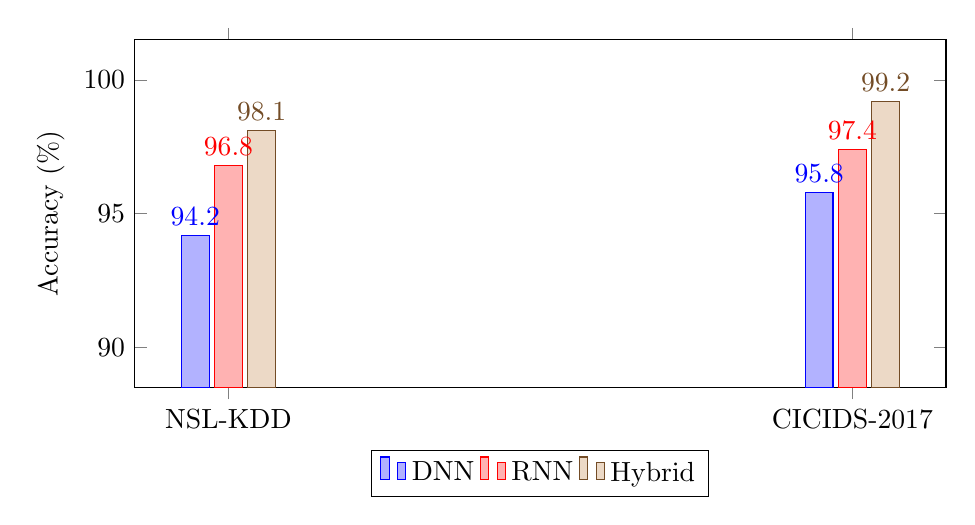
\begin{tikzpicture}
\begin{axis}[
    ybar,
    enlargelimits=0.15,
    legend style={at={(0.5,-0.18)},
      anchor=north,legend columns=-1},
    ylabel={Accuracy (\%)},
    symbolic x coords={NSL-KDD, CICIDS-2017},
    xtick=data,
    nodes near coords,
    nodes near coords align={vertical},
    ymin=90, ymax=100,
    width=0.98\linewidth,
    height=6cm
    ]
\addplot coordinates {(NSL-KDD,94.2) (CICIDS-2017,95.8)};
\addplot coordinates {(NSL-KDD,96.8) (CICIDS-2017,97.4)};
\addplot coordinates {(NSL-KDD,98.1) (CICIDS-2017,99.2)};
\legend{DNN, RNN, Hybrid}
\end{axis}
\end{tikzpicture}
\caption{Accuracy comparison showing overall classification success.}
\end{figure}

\begin{figure}[h]
\centering
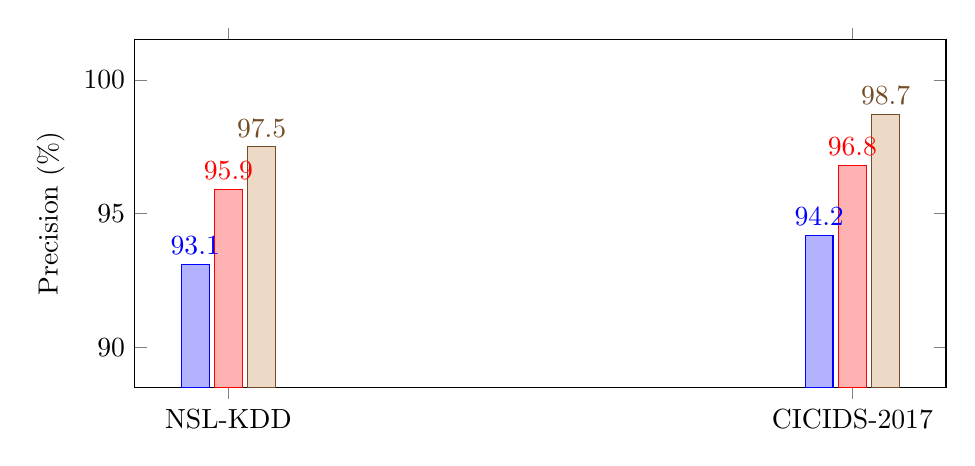
\begin{tikzpicture}
\begin{axis}[
    ybar,
    enlargelimits=0.15,
    ylabel={Precision (\%)},
    symbolic x coords={NSL-KDD, CICIDS-2017},
    xtick=data,
    nodes near coords,
    ymin=90, ymax=100,
    width=0.98\linewidth,
    height=6cm
    ]
\addplot coordinates {(NSL-KDD,93.1) (CICIDS-2017,94.2)};
\addplot coordinates {(NSL-KDD,95.9) (CICIDS-2017,96.8)};
\addplot coordinates {(NSL-KDD,97.5) (CICIDS-2017,98.7)};
\end{axis}
\end{tikzpicture}
\caption{Precision comparison demonstrating low False Positive Rates.}
\end{figure}

\begin{figure}[h]
\centering
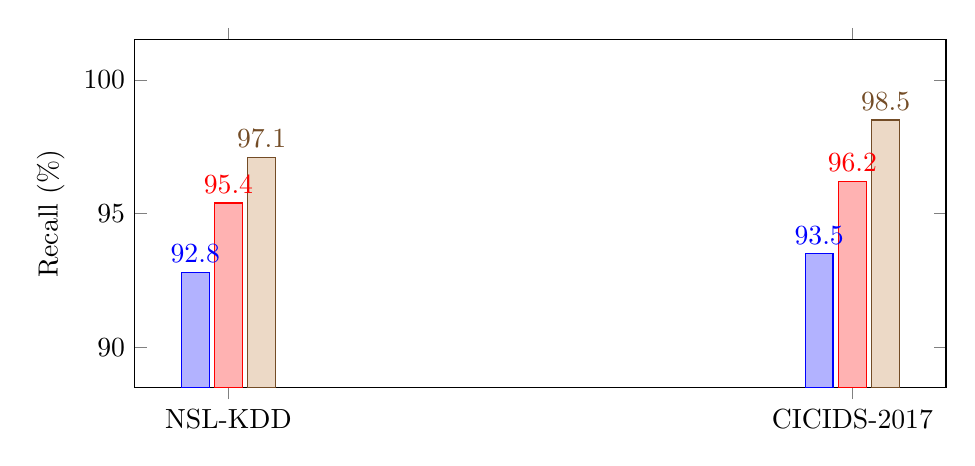
\begin{tikzpicture}
\begin{axis}[
    ybar,
    enlargelimits=0.15,
    ylabel={Recall (\%)},
    symbolic x coords={NSL-KDD, CICIDS-2017},
    xtick=data,
    nodes near coords,
    ymin=90, ymax=100,
    width=0.98\linewidth,
    height=6cm
    ]
\addplot coordinates {(NSL-KDD,92.8) (CICIDS-2017,93.5)};
\addplot coordinates {(NSL-KDD,95.4) (CICIDS-2017,96.2)};
\addplot coordinates {(NSL-KDD,97.1) (CICIDS-2017,98.5)};
\end{axis}
\end{tikzpicture}
\caption{Recall comparison highlighting detection of Malicious classes.}
\end{figure}

\begin{figure}[h]
\centering
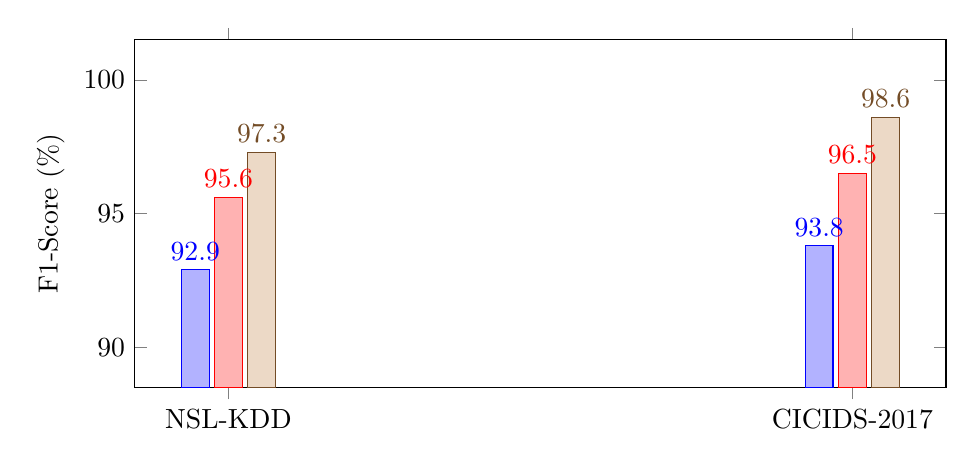
\begin{tikzpicture}
\begin{axis}[
    ybar,
    enlargelimits=0.15,
    ylabel={F1-Score (\%)},
    symbolic x coords={NSL-KDD, CICIDS-2017},
    xtick=data,
    nodes near coords,
    ymin=90, ymax=100,
    width=0.98\linewidth,
    height=6cm
    ]
\addplot coordinates {(NSL-KDD,92.9) (CICIDS-2017,93.8)};
\addplot coordinates {(NSL-KDD,95.6) (CICIDS-2017,96.5)};
\addplot coordinates {(NSL-KDD,97.3) (CICIDS-2017,98.6)};
\end{axis}
\end{tikzpicture}
\caption{F1-Score comparison showing the harmonic balance of metrics.}
\end{figure}

Taken together, the four plots emphasize two facts. First, every model exceeds the mid-nineties on headline metrics, so the experimental question is not whether learning-based detectors work on these benchmarks, but which architecture best preserves recall while keeping precision high. Second, the hybrid's advantage is most visible in recall and $F_1$, which are the metrics most sensitive to missed attacks and class skew.

\subsection{Class-Specific Recall: NSL-KDD Dataset}
NSL-KDD groups attacks into DoS, Probe, remote-to-local (R2L), and user-to-root (U2R) families. DoS and Probe are comparatively frequent and exhibit strong statistical regularity; R2L and U2R are sparser and closer to legitimate administrative activity, which historically causes weaker detectors to collapse toward benign predictions. The per-class recall chart should therefore be read as a stress test on the tail behavior of each model rather than as a second copy of the aggregate table.

Across models, DoS recall is already excellent for the DNN (96.2\%) and climbs modestly for the hybrid (98.9\%), which is expected when volumetric abuse dominates the feature space. The meaningful spread appears in R2L and U2R: the DNN attains 82.3\% and 78.1\% recall on those classes, the RNN improves them to 88.4\% and 82.5\%, and the hybrid reaches 91.2\% and 86.8\%. Those increments are consistent with giving the classifier both a rich per-flow embedding and a memory of recent related events, which is precisely where single-step dense models tend to underfit.

\begin{table}[h]
\centering
\caption{Class-Specific Recall (\%) on NSL-KDD by Attack Category}
\label{table:nsl_class_recall}
\begin{tabular}{|l|c|c|c|c|}
\hline
\textbf{Model} & \textbf{DoS} & \textbf{Probe} & \textbf{R2L} & \textbf{U2R} \\ \hline
DNN & 96.2 & 94.5 & 82.3 & 78.1 \\
RNN & 97.8 & 96.1 & 88.4 & 82.5 \\
\textbf{Hybrid} & \textbf{98.9} & \textbf{97.4} & \textbf{91.2} & \textbf{86.8} \\ \hline
\end{tabular}
\end{table}

\begin{figure}[h]
\centering
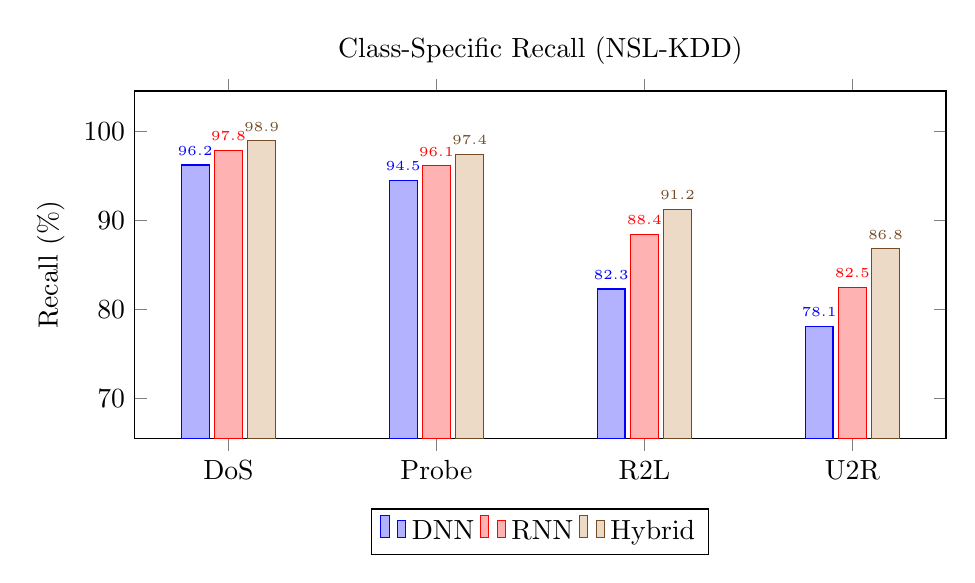
\begin{tikzpicture}
\begin{axis}[
    title={Class-Specific Recall (NSL-KDD)},
    ybar,
    enlargelimits=0.15,
    legend style={at={(0.5,-0.2)}, anchor=north, legend columns=-1},
    ylabel={Recall (\%)},
    symbolic x coords={DoS, Probe, R2L, U2R},
    xtick=data,
    ymin=70, ymax=100,
    width=0.98\linewidth,
    height=6cm,
    nodes near coords,
    every node near coord/.append style={font=\tiny}
    ]
\addplot coordinates {(DoS,96.2) (Probe,94.5) (R2L,82.3) (U2R,78.1)};
\addplot coordinates {(DoS,97.8) (Probe,96.1) (R2L,88.4) (U2R,82.5)};
\addplot coordinates {(DoS,98.9) (Probe,97.4) (R2L,91.2) (U2R,86.8)};
\legend{DNN, RNN, Hybrid}
\end{axis}
\end{tikzpicture}
\caption{Detection rates for legacy attack vectors in NSL-KDD.}
\end{figure}

The NSL-KDD figure therefore corroborates the aggregate story: hybridization is not only a marginal accuracy tweak; it reallocates probability mass toward rare classes that are easy to ignore when optimizing global loss.

\subsection{Class-Specific Recall: CICIDS-2017 Dataset}
On CICIDS-2017 we isolate DDoS, botnet, brute-force, and infiltration-style behaviors. DDoS again saturates quickly---the DNN already reaches 97.8\% recall---while botnet and brute-force attacks show moderate headroom between 92.5\% and 97.5\% recall depending on the model. Infiltration remains the hardest column: the DNN stops at 86.3\%, the RNN at 89.5\%, and the hybrid at 91.2\%. Although all scores are high in absolute terms, the infiltration gap is where temporal correlation and subtle feature interactions are most plausible, so the ordering supports the architectural narrative developed in Section~III.

\begin{table}[h]
\centering
\caption{Class-Specific Recall (\%) on CICIDS-2017 by Attack Category}
\label{table:cic_class_recall}
\begin{tabular}{|l|c|c|c|c|}
\hline
\textbf{Model} & \textbf{DDoS} & \textbf{Botnet} & \textbf{BruteForce} & \textbf{Infiltration} \\ \hline
DNN & 97.8 & 92.5 & 94.1 & 86.3 \\
RNN & 98.5 & 94.1 & 95.9 & 89.5 \\
\textbf{Hybrid} & \textbf{99.4} & \textbf{96.8} & \textbf{97.5} & \textbf{91.2} \\ \hline
\end{tabular}
\end{table}

\begin{figure}[h]
\centering
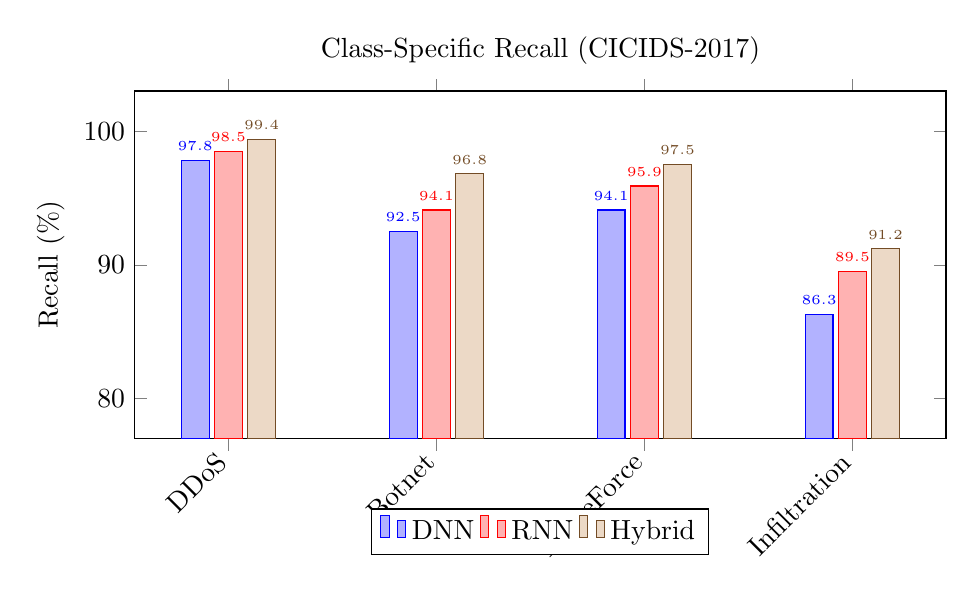
\begin{tikzpicture}
\begin{axis}[
    title={Class-Specific Recall (CICIDS-2017)},
    ybar,
    enlargelimits=0.15,
    legend style={at={(0.5,-0.2)}, anchor=north, legend columns=-1},
    ylabel={Recall (\%)},
    symbolic x coords={DDoS, Botnet, BruteForce, Infiltration},
    xtick=data,
    x tick label style={rotate=45, anchor=east},
    ymin=80, ymax=100,
    width=0.98\linewidth,
    height=6cm,
    nodes near coords,
    every node near coord/.append style={font=\tiny}
    ]
\addplot coordinates {(DDoS,97.8) (Botnet,92.5) (BruteForce,94.1) (Infiltration,86.3)};
\addplot coordinates {(DDoS,98.5) (Botnet,94.1) (BruteForce,95.9) (Infiltration,89.5)};
\addplot coordinates {(DDoS,99.4) (Botnet,96.8) (BruteForce,97.5) (Infiltration,91.2)};
\legend{DNN, RNN, Hybrid}
\end{axis}
\end{tikzpicture}
\caption{Recall performance on modern threat categories in CICIDS-2017.}
\end{figure}

Relative to NSL-KDD, CICIDS-2017 pushes recall upward across the board for modern high-volume attacks, yet the hardest class still benefits the most from the hybrid design. That observation grounds later deployment discussions: gains are unlikely to be uniform across every attack taxonomy, so evaluation must continue to stratify by family.

\section{Discussion of Strategic Findings}
The measurements in Section~IV support a straightforward systems interpretation. Dense feedforward layers are an efficient way to compress high-dimensional flow vectors into a decision boundary that separates obvious abuse from benign bulk traffic. Recurrent cells, by contrast, inject path-dependent structure that helps when malicious activity is distributed across several related flows or epochs. Neither mechanism alone is theoretically sufficient for every threat model; the hybrid stacks them so that spatial abstractions feed temporal inference, which is why the largest recall deltas concentrate in U2R, R2L, and infiltration-style categories instead of raw denial-of-service floods.

\subsection{The Spatial-Temporal Synergy}
The standalone DNN performs strongly whenever attack signatures manifest as sharp distributional shifts in engineered flow statistics, which is why DoS and DDoS recalls sit at the top of their respective charts. Those events dominate volume and leave a clear footprint in packet and timing aggregates. Infiltration and U2R are qualitatively different: they mimic legitimate administrative traffic, unfold slowly, and may rely on sequences of modest anomalies rather than a single spike. The standalone RNN recovers part of that structure but still trails the hybrid on several cells, suggesting that feeding an LSTM raw or weakly structured inputs limits how much temporal context it can exploit. The \textbf{hybrid model} closes most of that gap; on CICIDS-2017 infiltration recall, it improves by 4.9 percentage points over the DNN baseline (from 86.3\% to 91.2\%), cutting the DNN's missed-infiltration mass $(1-\text{recall})$ by more than one third in relative terms. That is a meaningful shift for an analyst queue because infiltration alarms are inherently sparse and high stakes.

\subsection{Operational Feasibility and False Positives}
Precision is the practical counterpart to recall in a security operations center: a model that surfaces too many false positives will be tuned down, whitelisted aggressively, or ignored, which indirectly raises the false-negative rate in production. The hybrid model's 98.7\% precision on CICIDS-2017, paired with its highest recall in Table~\ref{table:overall_metrics}, indicates that the observed recall gains are not purchased through indiscriminate alerting. Latency is also a deployment constraint rather than a laboratory curiosity. At roughly 1.6\,ms per flow on GPU-class hardware, the hybrid is slower than a hash lookup but still compatible with online scoring on aggregated flows when batching and hardware offload are available; signature engines and learning-based tiers therefore remain complementary instead of mutually exclusive.

\section{Conclusion}
This paper examined deep learning as a mechanism for reducing reliance on static malware and intrusion signatures in the face of zero-day and polymorphic threats. Using NSL-KDD and CICIDS-2017, we compared dense, recurrent, and hybrid architectures under a common preprocessing and evaluation protocol. Across both datasets, the hybrid DNN--RNN model achieved the strongest overall accuracy, precision, recall, and $F_1$ score, with the most pronounced per-class recall improvements on low-rate privilege-escalation and infiltration behaviors where temporal correlation plausibly carries explanatory signal. These findings do not imply that neural detectors replace curated rules; rather, they suggest that a hybrid spatial--temporal learner can prioritize nuanced cases for human review while leaving obvious bulk attacks to fast path defenses.

\section{Future Work}
Several extensions would tighten the scientific and engineering claims beyond benchmark scoring. First, we plan to evaluate continuity under realistic domain shift by training on one campus or cloud trace and testing on another, measuring degradation in precision and recall over time \cite{sommer2010}. Second, newer corpora such as CSE-CIC-IDS2018 and enterprise-specific captures should be incorporated so that results are not tied to a single generation of labeling tooling \cite{hindy2020}. Third, adversarial robustness and data-poisoning defenses must be treated as first-class requirements because attackers increasingly optimize against learned detectors \cite{biggio2018,yuan2019}; adversarial training, input sanitization, and integrity controls on training pipelines are natural next steps. Fourth, operational integration paths---including calibrated probabilities, cost-sensitive thresholds per asset class, and feedback loops from analyst disposition---need empirical study so that model scores translate into sustainable workflows rather than static leaderboard numbers. Finally, privacy-preserving training strategies (e.g., federated or differentially private updates) warrant investigation before wide deployment on sensitive traffic metadata.

\section*{Acknowledgment}
The authors thank the University of Central Florida Department of Computer Science for resources and support for this course project. The authors are grateful to Dr.~Cliff for his instruction and guidance throughout this project.

\begin{thebibliography}{00}
\bibitem{buczak2016} A. L. Buczak and E. Guven, "A Survey of Data Mining and Machine Learning Methods for Cyber Security," in IEEE Communications Surveys \& Tutorials, vol. 18, no. 2, pp. 1153--1176, 2016.
\bibitem{denning1987} D. E. Denning, "An Intrusion-Detection Model," in IEEE Trans. Software Eng., vol. SE-13, no. 2, pp. 222--232, Feb. 1987.
\bibitem{idika2007} N. Idika and M. Mathur, "A Survey of Malware Detection Techniques," Purdue University, Tech. Rep., 2007.
\bibitem{alshamrani2019} A. Alshamrani et al., "A Survey on Advanced Persistent Threats: Techniques, Solutions, Challenges, and Efforts," in IEEE Communications Surveys \& Tutorials, vol. 21, no. 2, pp. 1851--1877, 2019.
\bibitem{axelsson2000} S. Axelsson, "The Base-Rate Fallacy and the Difficulty of Intrusion Detection," in ACM Trans. Inf. Syst. Secur., vol. 3, no. 3, pp. 186--205, 2000.
\bibitem{lecun2015} Y. LeCun, Y. Bengio, and G. Hinton, "Deep Learning," Nature, vol. 521, no. 7553, pp. 436--444, 2015.
\bibitem{sharafaldin2018} I. Sharafaldin, A. H. Lashkari, and A. A. Ghorbani, "Toward a Reliable Dataset for Intrusion Detection," in Proc. ICISSP, 2018.
\bibitem{sommer2010} R. Sommer and V. Paxson, "Outside the Closed World: On Using Machine Learning for Network Intrusion Detection," in Proc. IEEE S\&P, 2010.
\bibitem{kim2016} J. Kim et al., "Long Short-Term Memory RNN for Intrusion Detection," in Proc. PlatCon, 2016.
\bibitem{yin2017} C. Yin et al., "A Deep Learning Approach for IDS Using RNNs," IEEE Access, 2017.
\bibitem{tavallaee2009} M. Tavallaee et al., "A detailed analysis of the KDD CUP 99 data set," in Proc. IEEE CISDA, 2009.
\bibitem{ferrag2020} M. A. Ferrag et al., "Deep Learning for Cyber Security In Situ and In Transit: A Survey," IEEE Communications Surveys \& Tutorials, 2020.
\bibitem{hindy2020} H. Hindy et al., "A Taxonomy and Survey of Intrusion Detection System Datasets," IEEE Access, 2020.
\bibitem{zhang2019} Y. Zhang et al., "A Hierarchical DL Approach for Intrusion Detection," ACM Trans. Intell. Syst. Technol., 2019.
\bibitem{javaid2016} A. Javaid et al., "A Deep Learning Approach for Network Intrusion Detection System," in Proc. ICACCI, 2016.
\bibitem{otoum2019} S. Otoum et al., "Empowering IDS with Deep Learning in IoT," IEEE Communications Magazine, 2019.
\bibitem{biggio2018} B. Biggio and F. Roli, "Wild Patterns: Ten Years After the Rise of Adversarial Machine Learning," Pattern Recognition, 2018.
\bibitem{yuan2019} X. Yuan et al., "Adversarial Examples: Attacks and Defenses for Deep Learning," IEEE Trans. Neural Netw. Learn. Syst., 2019.
\end{thebibliography}

\end{document}